\documentclass[12pt]{article}
\usepackage{graphicx}%Package um Grafiken einzufügen
\graphicspath{ {assets/} }
\usepackage[ngerman]{babel}%Sprache Deutsch einstellen
\usepackage[headheight=15pt, a4paper, left=40mm, top=20mm, bottom=20mm, right=20mm]{geometry}
\usepackage[]{fontspec}
\setmonofont{CascadiaCode.ttf}[Scale=0.88]
\usepackage[]{fancyhdr}
\pagestyle{fancy}
%\setlength{\headheight}{16pt}
\lhead{\leftmark}
\rhead{Phillip Bronzel} 

\usepackage[style=authoryear, backend=biber]{biblatex}
\addbibresource{references.bib}
\usepackage{csquotes}

\usepackage{eso-pic}
\newcommand\BackgroundPic{
    \put(0,0){
    \parbox[b][\paperheight]{\paperwidth}{
    \vfill
    \centering
    
\includegraphics[width=\paperwidth,height=\paperheight]{assets/titlebackground.pdf}
    \vfill
    }}}

\usepackage{chronology}

\usepackage{subfig}

\usepackage{pgfplots}

\usepackage[onehalfspacing]{setspace}

\usepackage[bottom]{footmisc}

\usepackage{wrapfig}

\usepackage{xcolor}

\usepackage{float}

\usepackage{minted}
\usemintedstyle{pastie}
\renewcommand\listoflistingscaption{Quellcodeverzeichnis}

\usepackage{amsmath}

\usepackage{tikz}
\usetikzlibrary{matrix,calc,arrows.meta,bending}

\usepackage{ifthen}

\setcounter{secnumdepth}{3} \setcounter{tocdepth}{4}

\title{Machine Learning in Smartphone Apps}
\date{Phillip Bronzel \today}
\author{ASGSG Informatik, 2020/2021}

\begin{document}
\AddToShipoutPicture*{\BackgroundPic}
\maketitle
\pagenumbering{gobble}
\begin{center}
    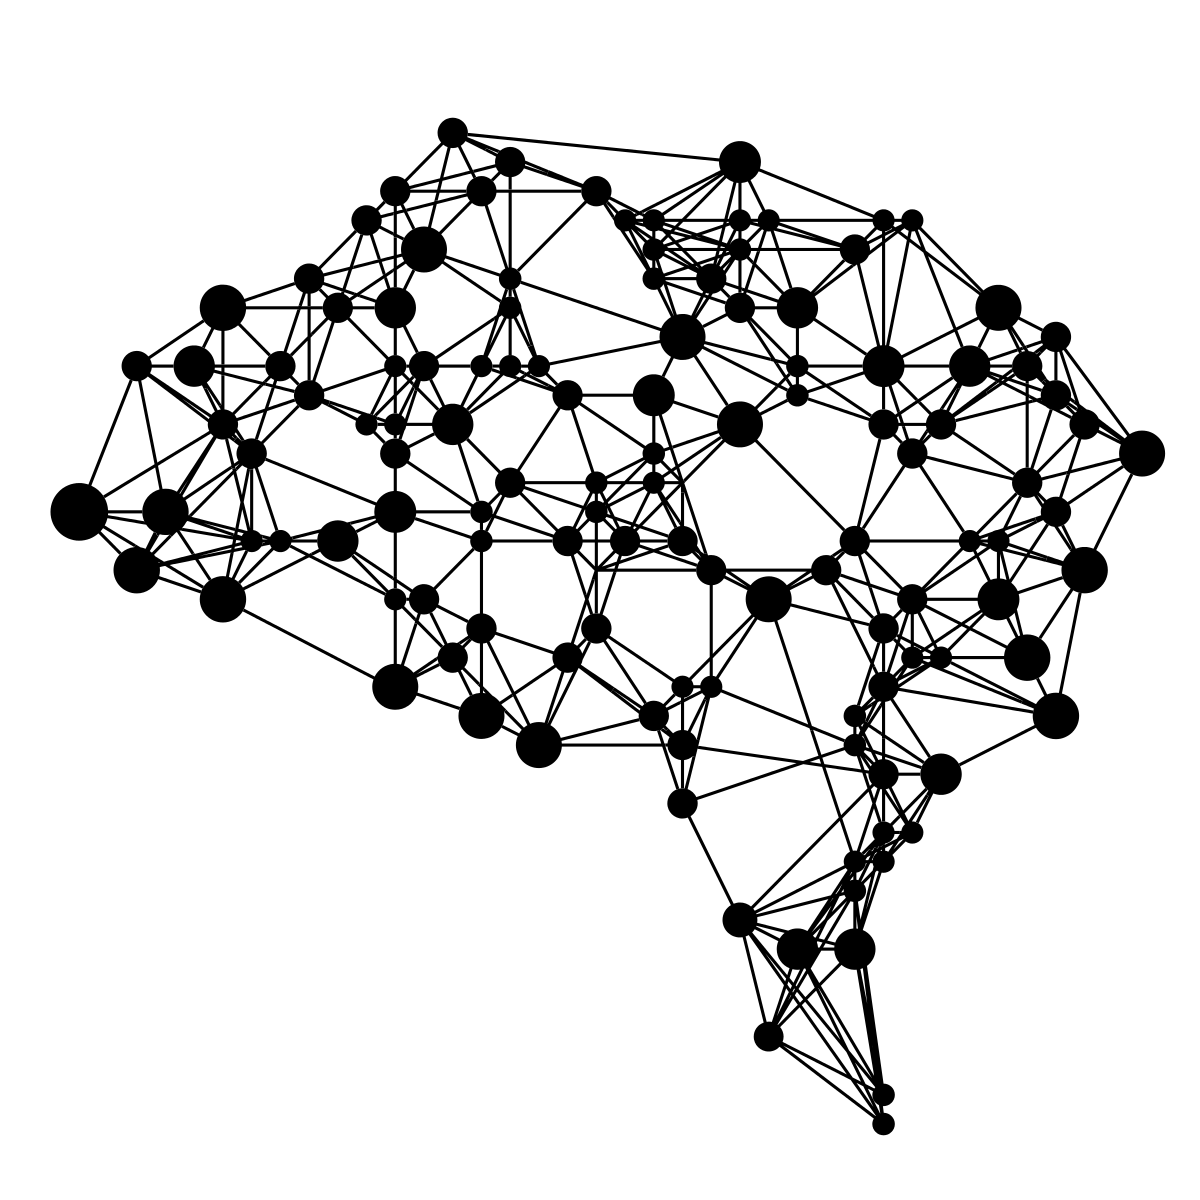
\includegraphics[totalheight=10cm]{titlepage.png}
    \cite{titlepageimage}
\end{center}

\input{lib/erklärung.tex}

\newpage
\pagenumbering{arabic}
\tableofcontents

\newpage
\input{lib/einführung.tex}%TODO: Kapitel der App einfügen

\section{Neuronale Netzwerke}

\subsection{Geschichte}

Im Jahr 1943 wurde die erste Arbeit darüber geschrieben, wie Neuronen im Gehirn funktionieren könnten und die Autoren Warren McCulloch und Walter Pitts experimentierten sogar damit diese mit elektronischen Schaltkreisen nachzubauen.\footnote[6]{\cite[]{alogicalcalculus}} In den 1950er Jahren haben Forscher von IBM daran gearbeitet ein NN\footnote[7]{Kurzform für Neuronales Netzwerk, wird ab jetzt weiterhin verwendet.} mit einem Computer zu simulieren. Der Versuch scheiterte allerdings.\footnote[8]{\cite[Absatz 3]{nnhistory}} Immer wieder gab es kleinere Forschungsprojekte, ein sehr großer Durchbruch war aber 1975 die Entwicklung eines "`Backpropagation"' Algorithmus durch den Wissenschaftler Paul Werbos. Ähnliche Algorithmen wurden wiederholt und unabhängig entwickelt, aber Werbos' Algorithmus war der erste mit großer Bedeutung.\footnote[9]{\cite[]{paulwerbosbackpropagation}} Das Prinzip des Algorithmus wird auch heute noch verwendet, es ist dieser Algorithmus der dem Neuronalen Netzwerk das selbstständige Lernen ermöglicht.\footnote[10]{siehe Kapitel \ref{funktionsweise}}
\subsubsection{Zeitstrahl}

\begin{chronology}[10]{1940}{2020}{\textwidth}
    \event{1943}{Erste Arbeit und Experimente}
    \event[1950]{1960}{Bemühungen, ein NN digital umzusetzen}
    \event{1975}{Backpropagation Algorithmus}
\end{chronology}

\subsection{Aufbau}

\begin{center}
    \begin{tikzpicture}[x=1.5cm, y=1.5cm, >=stealth]

        \foreach \m/\l [count=\y] in {1,2,3,missing,4}
        \node [every neuron/.try, neuron \m/.try] (input-\m) at (0,2.5-\y) {};

        \foreach \m [count=\y] in {1,missing,2}
        \node [every neuron/.try, neuron \m/.try ] (hidden-\m) at (2,2-\y*1.25) {};

        \foreach \m [count=\y] in {1,missing,2}
        \node [every neuron/.try, neuron \m/.try ] (output-\m) at (4,1.5-\y) {};

        \foreach \l [count=\i] in {1,2,3,n}
        \draw [<-] (input-\i) -- ++(-1,0)
        node [above, midway] {$I_\l$};

        \foreach \l [count=\i] in {1,n}
        \node [above] at (hidden-\i.north) {$H_\l$};

        \foreach \l [count=\i] in {1,n}
        \draw [->] (output-\i) -- ++(1,0)
        node [above, midway] {$O_\l$};

        \foreach \i in {1,...,4}
        \foreach \j in {1,...,2}
        \draw [->] (input-\i) -- (hidden-\j);

        \foreach \i in {1,...,2}
        \foreach \j in {1,...,2}
        \draw [->] (hidden-\i) -- (output-\j);

        \foreach \l [count=\x from 0] in {Eingabe, Versteckte, Ausgangs}
        \node [align=center, above] at (\x*2,2) {\l \\ Ebene};

    \end{tikzpicture}
\end{center}

\subsection{Funktionsweise} \label{funktionsweise}

\subsubsection{Trainieren - Backpropagation}

\newpage
\appendix
\label{Anhang}
\section{Anhang}

\subsection{Weitere Aktivierungsfunktionen}\label{anhang:weitereaktivierungsfunktionen}

\begin{figure}[h]
    \center
    \begin{tikzpicture}
    \begin{axis}
        [
            grid=major,
            xmin=-3,
            xmax=3,
            axis x line=bottom,
            ytick={0,1,2},
            ymax=2.5,
            ymin=-0.5,
            axis y line=middle,
            legend style={at={(0.5,-0.2)},anchor=north}
        ]
        \addplot[red,mark=none]{(x>=0)*x};
        \addplot[blue, mark=none]{0.5*(tanh(\x)+1)};
        \legend{ReLU - $\max{(0,x)}$, (Verschobene) Hyperbolische Tangente - $0.5(\tanh{(x)}+1)$}
    \end{axis}
\end{tikzpicture}
    \caption[Aktivierungsfunktionen]{Weitere Aktivierungsfunktionen, ergänzend zu der Sigmoid Funktion aus Kapitel \ref{funktionsweise}}
    \label{Aktivierungsfunktionen}%
\end{figure}

Die ReLU (Rectified linear Unit) Funktion ist im Vergleich zu anderen Aktivierungsfunktionen, wie der Sigmoidfunktion oder der Hyperbolischen Tangente, deutlich simpler, was sich in Leistungsansprüchen des Trainingsprozesses wiederspiegelt.\footnote{\cite{nnfs}}

\subsection{Code für das Beispiel aus \ref{funktionsweise}}\label{anhang:colab1}

\begin{listing}[H]
    \begin{minted}[fontsize=\footnotesize,linenos]{python}
import tensorflow as tf
import tensorflow.keras.layers as layers

numberOfNeuronsInFirstLayer = 16 
numberOfNeuronsInSecondLayer = 16 
numOfEpochs = 5 

mnist = tf.keras.datasets.mnist

(x_train, y_train), (x_test, y_test) = mnist.load_data() # Laden des MNIST Datasets
# Und aufteilen in Trainigsdaten und Testdaten

x_train = tf.keras.utils.normalize(x_train, axis=1) # Normalisieren des Datasets
x_test = tf.keras.utils.normalize(x_test, axis=1)

model = tf.keras.models.Sequential() # Erstellen des Neuronalen Netzwerks
model.add(layers.Flatten())
model.add(layers.Dense(numberOfNeuronsInFirstLayer, activation=tf.nn.sigmoid))
# Hinzufügen der Layer
model.add(layers.Dense(numberOfNeuronsInSecondLayer, activation=tf.nn.sigmoid))
model.add(layers.Dense(10, activation=tf.nn.softmax))

model.compile(optimizer='adam',
              loss='sparse_categorical_crossentropy',
              metrics=['accuracy']) # Kompilieren der Layer zu einem trainierfähigen Modell

model.fit(x_train, y_train, epochs=numOfEpochs)
# Trainieren des Modells mit den Trainingsdaten und x Epochen

model.save('beispielModel_MNIST') # Speichern des Modells

    \end{minted}
    \caption{Umsetzung mit Python und Tensorflow}
\end{listing}
Ein interaktives Beispiel gibt es zusätzlich hier in meinem Colab Notebook: \url{https://bit.ly/34Ggfuh}\footnote{Ungekürzter Link: \url{https://colab.research.google.com/drive/1ty_QQlL038YT6KpBjSdqGvIGyH0YXwxW}}

\subsection{Labelcheck Code}\label{anhang:labelchecktf}

asdf

\subsection{Die Flutter Architektur}\label{anhang:flutterarc}

\begin{figure}[H]
    \centering
    \resizebox{\textwidth}{!}{
    \includesvg{assets/flutterarchitecture}
    }
    \caption{Flutter's Architektur (\cite{flutterarchitecture})}
\end{figure}

Flutters Architektur ist in drei Ebenen unterteilt. Als Basis die "`Embedder Ebene"', welche für jede Platform angepasst werden muss und zum Beispiel für das Thread Management zuständig ist. Dadrüber liegt die "`Engine Ebene"', welche zu einem Großteil in C++ geschrieben ist und zu welcher auch die Grafikengine Skia gehört. Dadrüber liegt die "`Framework Ebene"', welche zum Beispiel die UI Komponenten beinhaltet und komplett in Dart entwickelt wird.\footnote{\cite{flutterarchitecture}}

\newpage
\printbibliography[heading=bibintoc, title={Literaturverzeichnis}]

\end{document}